	\subsection{Taxonomy of virtualization concepts by \textit{Pék}}
	
	\begin{figure}[!hbtp]
		\centering
		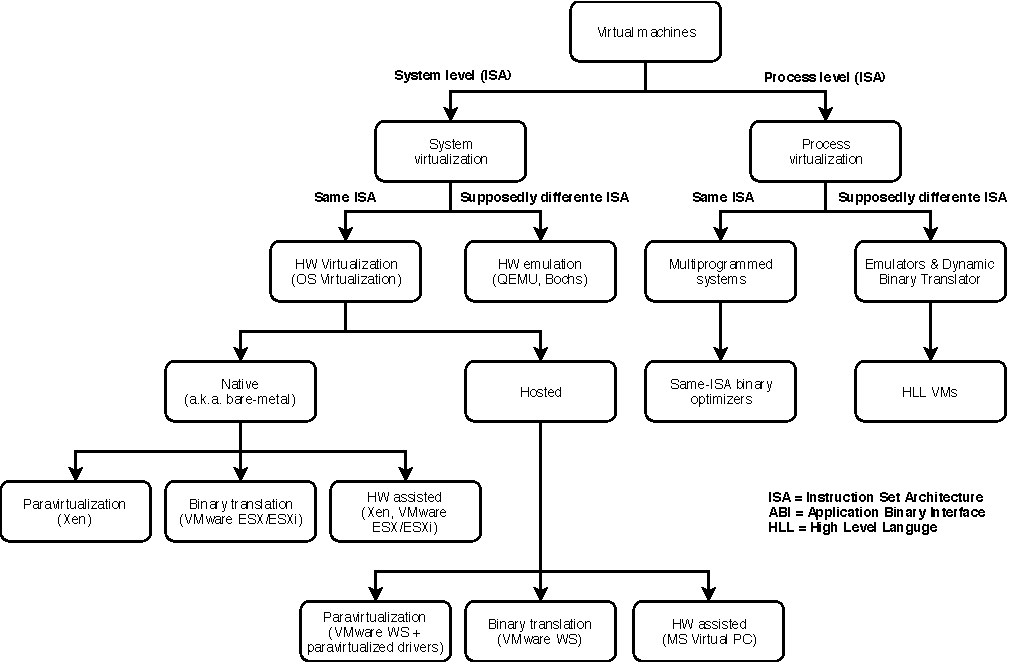
\includegraphics[width=9cm]{images/Pek2013.pdf}
		\vspace{-0.2cm}
		\caption{Taxonomy of virtualization concepts by \textit{Gábor Pék et al.} in 2013\footnotemark[9]{}.}
		\label{fig:TaxonomyOfVirtualizationConcepts}
	\end{figure}
	
	\footnotetext [9] {Figure bases on the study \textit{A Survey of Security Issues in Hardware Virtualization} by Pék Gábor, Buttyán Levente and Bencsáth Boildizsár, in 2013.}
	
	In 2013, \textit{Pék et al.} \cite{Pek2013} published research that includes a taxonomy of virtualization concepts. This study corresponds to an extension of the preliminary research by \textit{Smith} and \textit{Nair} in 2005 \cite{Smith2005}, and the \textit{SCOPE Alliance} in 2008 \cite {SCOPEAlliance2008}, see Figure \ref{fig:TaxonomyOfVirtualizationConcepts}. This contribution considers additional elements and the inclusion of several examples, particularly in the\textit{Hosted} category, which is equivalent to Type-2 hypervisors from the \textit{SCOPE Alliance} study. This taxonomy includes the subcategories of \textit{Para-virtualization} (VMware Workstation + Para-virtualization drivers), \textit{Binary translation} (VMware Workstation) and \textit{Hardware-assisted} (Microsoft Virtual PC). The other elements of the taxonomy follow the distribution originally proposed by the study of \textit{Smith} and \textit {Nair} in 2005. \\
	
	Although \textit{Pék's} study presents a necessary extension to the previous reserch by the \textit{SCOPE Alliance} in 2008 \cite{SCOPEAlliance2008}, on the other hand, it shows a representation with less detail in the \textit{Process VMs} category, similar to \textit{Smit} and \textit{Nair}'s study in 2005 \cite{Smith2005}. Therefore, this taxonomy leaves a gap in the search for the details for the categorization of virtualization technologies. This is because, they are based on the above mentioned works, and they still have their limitations, since they do not contemplate the levels of abstraction in which virtualization technologies take place.